\documentclass{book}
 
%Russian-specific packages
%--------------------------------------
\usepackage[T2A]{fontenc}
\usepackage[utf8]{inputenc}
\usepackage[russian]{babel}
\usepackage{amsmath}
\usepackage{amssymb}
%--------------------------------------
 
%Hyphenation rules
%--------------------------------------
\usepackage{hyphenat}
\hyphenation{ма-те-ма-ти-ка вос-ста-нав-ли-вать доп-пель-ган-гер}
%--------------------------------------
 
\usepackage{graphicx}
\begin{document}
 
%\tableofcontents

\chapter[Что такое не везёт: p-values]{Что такое не везёт и как это рассчитывать: p-values}

\section*{Cтатистическая значимость}

Словосочетание <<статистическая значимость>> (или его психологического доппельгангера, <<достоверность>>), наверное, слышали все. Медицина, генетика, опросы про зубную пасту и против зубной пасты - весь этот поток информации обычно формализуется через понятие значимости. 

\begin{figure}
    \centering
    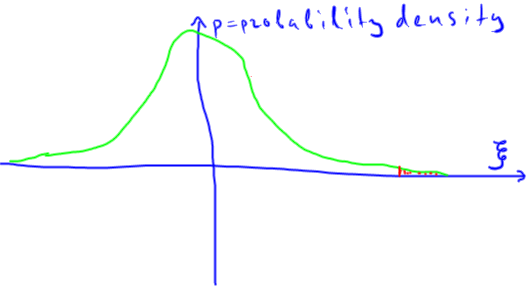
\includegraphics[scale=.5]{img/p-value.png}
    \caption{Площадь красного сегмента графика плотности вероятности случайной величины $\xi$ - это p-value, соответствующее значинию $\xi$ на границе сегмента}
    \label{pval}
\end{figure}



 
\end{document}
